\section{Introduction}
\subsection{Motivation and Background}
Since the Fortran 2008 standard (published in 2010~\cite{iso2010fortran}), Fortran supports a \gls{spmd} programming style
that facilitates the creation of a fixed number of replicas of a compiled program that execute asynchronously after a program
initiation.  Fortran refers to each replica as an image.  The primary mechanism for distributing and communicating data between
images involves defining \glspl{coarray}, an entity that may be referenced or defined on one image by statements executing on
other images. As such, a coarray defines a \gls{pgas}.

The seminal role that \gls{coarray} played in the development of Fortran's intrinsic parallel programming model have made it
common to refer to all of Fortran's parallel programming features under the rubric of ``\gls{caf}.''  To date, most applications
of \gls{caf} involve applications where the parallelization itself poses one of the chief challenges and custom parallel
parallel algorithms must be developed~\cite{preissl2011multithreaded,garain2015comparing,mozdzynski2015partitioned}.  In such settings, the moniker \gls{caf} seems appropriate as much of the parallel programming effort centers around expressing the algorithm in \gls{coarray} syntax.

Less widely appreciated is the role that Fortran may play in embarassingly parallel applications for which the upcoming
Fortran 2015 standard (to be published in 2018\footnote{A Committee Draft is at https://bit.ly/fortran-2015-draft.}) will
will provide several useful features.  These include the ability to declare teams of images that communicate with each other
by default and collective subroutines that enable compiler and parallel runtime library developers to offer highly optimized
implementations of common communication patterns such as broadcasts and reductions.

Fortran 2015 might well meet the parallel algorithmic needs of embarassingly parallel applications without the need to declare
any \glspl{coarray}.  A common use case will involve conducting an ensemble of simulations, each of which executes in a separate
image team and with any communication occuring in the collective subroutines provided by the new standard.  This paper presents
such a use case for a terrestrial hydrological model developed at \gls{ncar}: the \gls{wrf-hydro}.  For this work, we wrote
what we believe is the first implementation of compiler support for teams.  In addition to providing an open-source capability
for studying the teams features defined in the draft Fortran 2015 standard, our implementation offers a language extension
that is intended to facilitate the incremental introductionof \gls{caf} in an already functioning \gls{mpi} application.

\subsection{Objectives}

\section{Methodology}
\subsection{Teams implementation in GNU Fortran}
\subsection{Teams support in OpenCoarrays}
\subsection{Teams use in WRF-Hydro}

\section{Discussion of Results}

\section{Conclusions}

\begin{figure*}
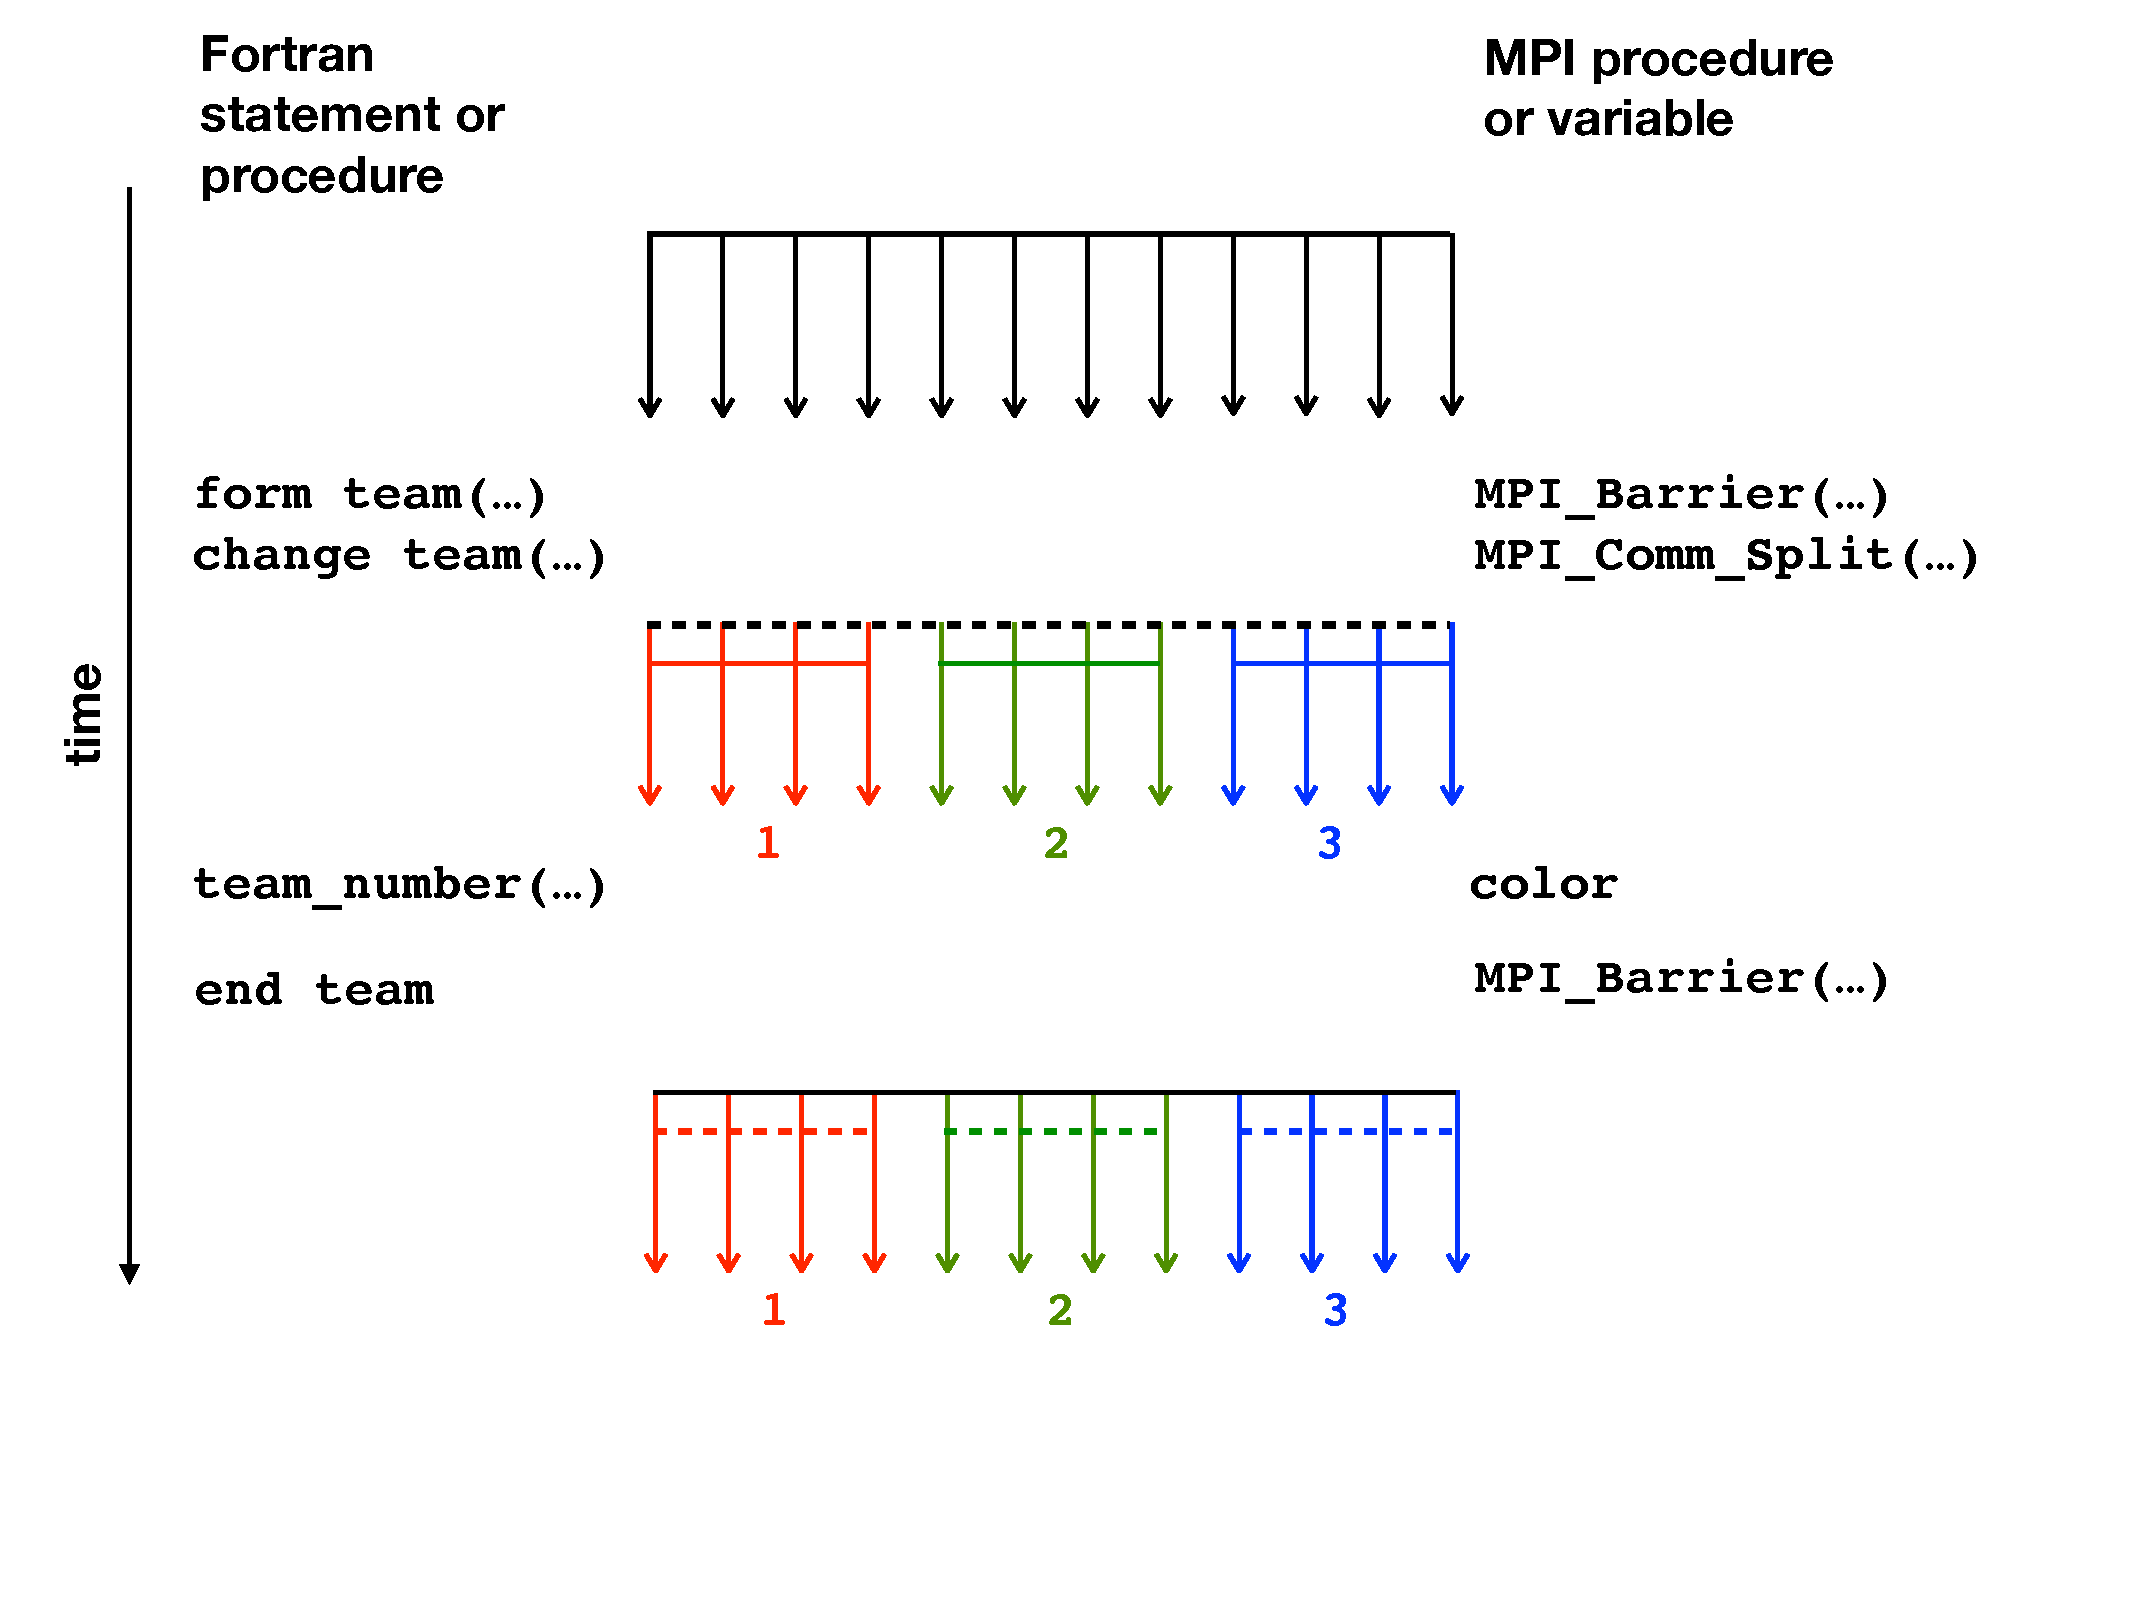
\includegraphics[width=0.7\textwidth]{figures/teams}
\vspace{-36pt}
\caption{Schematic depiction of a Fortran program executing over time (left axis) in 12 images (top) thatcommunicate with each other through global means (black horizontal bar) and later communicating within subgroups (colored horizontal bars).  Horizontal lines represent the communication mechanisms (default=solid, optional=dashed).  Fortran concepts or on the left.  The underlying \gls{mpi} concepts are the right.}
\end{figure*}
%

\begin{figure*}
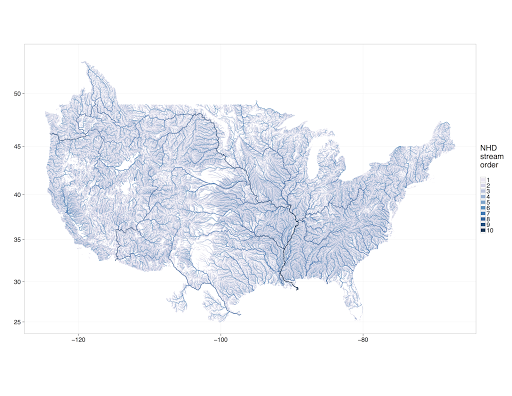
\includegraphics[width=0.7\textwidth]{figures/hydro-map}
\vspace{-36pt}
\caption{Sample WRF-Hydro simulation domain.}
\end{figure*}
%

%%%
%%% Sample tables
%%%

%\begin{table}
%  \caption{Frequency of Special Characters}
%  \label{tab:freq}
%  \begin{tabular}{ccl}
%    \toprule
%    Non-English or Math&Frequency&Comments\\
%    \midrule
%    \O & 1 in 1,000& For Swedish names\\
%    $\pi$ & 1 in 5& Common in math\\
%    \$ & 4 in 5 & Used in business\\
%    $\Psi^2_1$ & 1 in 40,000& Unexplained usage\\
%  \bottomrule
%\end{tabular}
%\end{table}

%\begin{table*}
%  \caption{Some Typical Commands}
%  \label{tab:commands}
%  \begin{tabular}{ccl}
%    \toprule
%    Command &A Number & Comments\\
%    \midrule
%    \texttt{{\char'134}author} & 100& Author \\
%    \texttt{{\char'134}table}& 300 & For tables\\
%    \texttt{{\char'134}table*}& 400& For wider tables\\
%    \bottomrule
%  \end{tabular}
%\end{table*}
% end the environment with {table*}, NOTE not {table}!

%It is strongly recommended to use the package booktabs~\cite{Fear05}
%and follow its main principles of typography with respect to tables:
%\begin{enumerate}
%\item Never, ever use vertical rules.
%\item Never use double rules.
%\end{enumerate}
%It is also a good idea not to overuse horizontal rules.


%%%
%%% Sample figures
%%%

%\begin{figure}
%\includegraphics{fly}
%\caption{A sample black and white graphic.}
%\end{figure}

%\begin{figure}
%\includegraphics[height=1in, width=1in]{fly}
%\caption{A sample black and white graphic
%that has been resized with the \texttt{includegraphics} command.}
%\end{figure}

%\begin{figure*}
%\includegraphics{flies}
%\caption{A sample black and white graphic
%that needs to span two columns of text.}
%\end{figure*}
%
%\begin{figure}
%\includegraphics[height=1in, width=1in]{rosette}
%\caption{A sample black and white graphic that has
%been resized with the \texttt{includegraphics} command.}
%\end{figure}

%\end{document}  % This is where a 'short' article might terminate



\appendix
%Appendix A
\section{Code listing}
% This next section command marks the start of
% Appendix B, and does not continue the present hierarchy
\section{Anything else?}

\begin{acks}
  The authors would like to thank the CISL and RAL Visitor Program

  The work is
  supported by the \grantsponsor{GSxxxxx}{National
  Science Foundation China}{http://dx.doi.org/zz.yyyyy/xxxxx} under Grant
  No.:~\grantnum{GSxxxxx}{yyyyyyy}

\end{acks}
